% inspired from http://tex.stackexchange.com/questions/63612/tikz-tree-drawing-with-comments-to-each-level and http://tex.stackexchange.com/questions/45808/tikz-grid-lines
\documentclass{article}

\usepackage{tikz}
\usetikzlibrary{trees}

\begin{document}

% Appels récursifs fibonacci

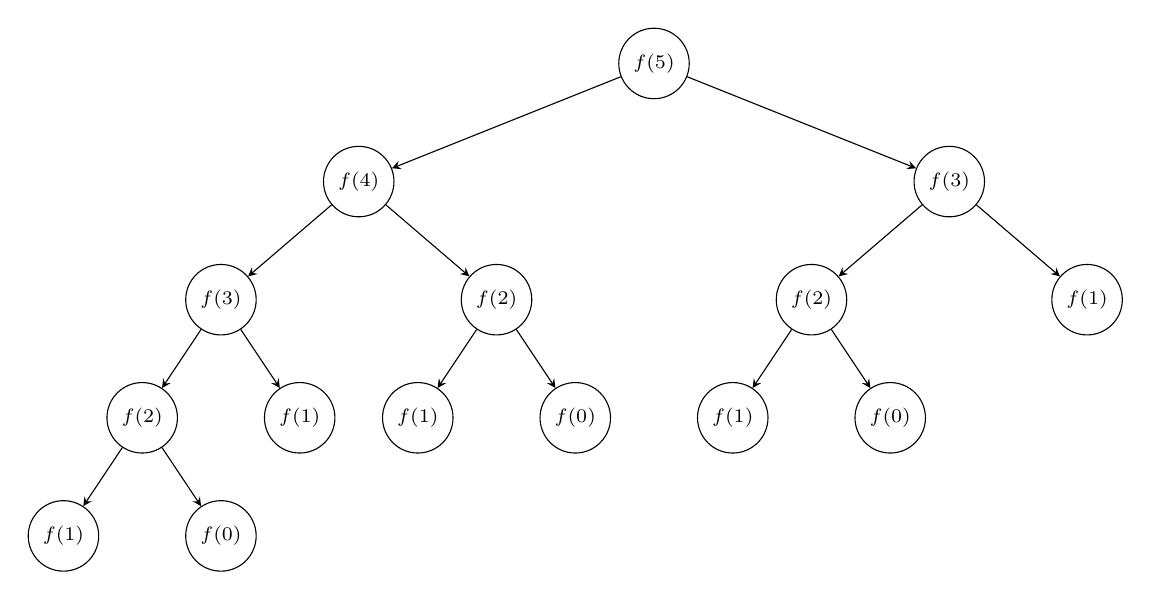
\begin{tikzpicture}[level distance = 1.5cm,
         level 1/.style = {->, >=stealth, sibling distance = 7.5cm},
         level 2/.style = {->, >=stealth, sibling distance = 3.5cm},
         level 3/.style = {->, >=stealth, sibling distance = 2cm},
         level 4/.style = {->, >=stealth, sibling distance = 2cm}]
\tikzstyle{every node} = [circle, draw, font = \sffamily\scriptsize]
\node (Root) {$f(5)$}
   child {
      node {$f(4)$}
      child { 
         node {$f(3)$}
         child { 
            node {$f(2)$}
            child { node {$f(1)$} }
            child { node {$f(0)$} }
         }
         child { node {$f(1)$} }
      }
      child { 
         node {$f(2)$}
         child { node {$f(1)$} }
         child { node {$f(0)$} }
      }
   }
   child {
      node {$f(3)$}
      child { 
         node {$f(2)$}
         child { node {$f(1)$} }
         child { node {$f(0)$} }
      }
      child { node {$f(1)$} }
   };

\end{tikzpicture}

% Appels récursifs fibonacci (version dynamique)

\vspace{1cm}

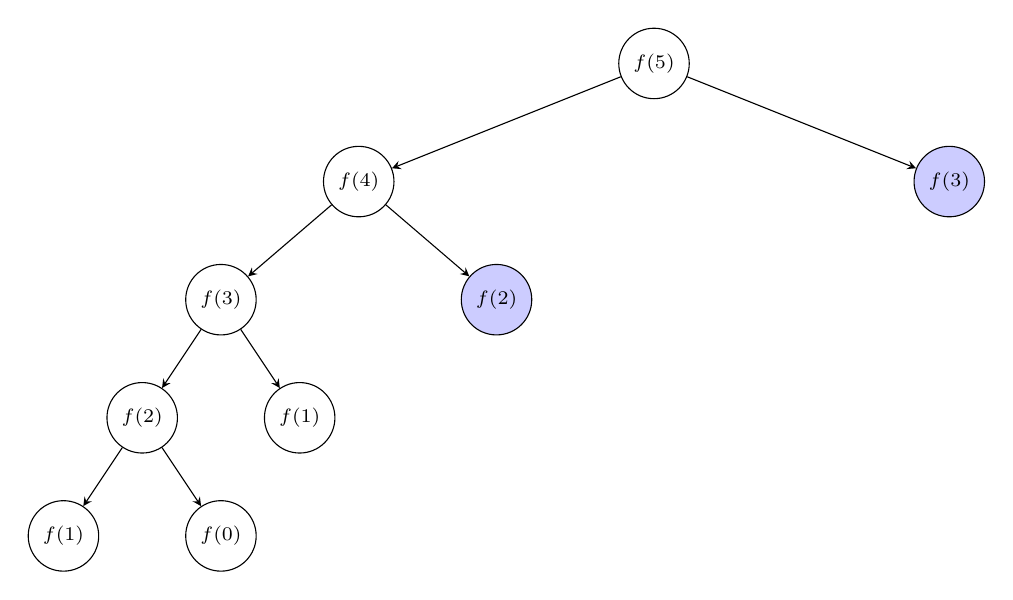
\begin{tikzpicture}[level distance = 1.5cm,
         level 1/.style = {->, >=stealth, sibling distance = 7.5cm},
         level 2/.style = {->, >=stealth, sibling distance = 3.5cm},
         level 3/.style = {->, >=stealth, sibling distance = 2cm},
         level 4/.style = {->, >=stealth, sibling distance = 2cm}]
\tikzstyle{every node} = [circle, draw, font = \sffamily\scriptsize]
\node (Root) {$f(5)$}
   child {
      node {$f(4)$}
      child { 
         node {$f(3)$}
         child { 
            node {$f(2)$}
            child { node {$f(1)$} }
            child { node {$f(0)$} }
         }
         child { node {$f(1)$} }
      }
      child { node [fill = blue!20] {$f(2)$} }
   }
   child { node [fill = blue!20] {$f(3)$} };

\end{tikzpicture}

% Comparaison méthodes ascendante et descendante

\newpage

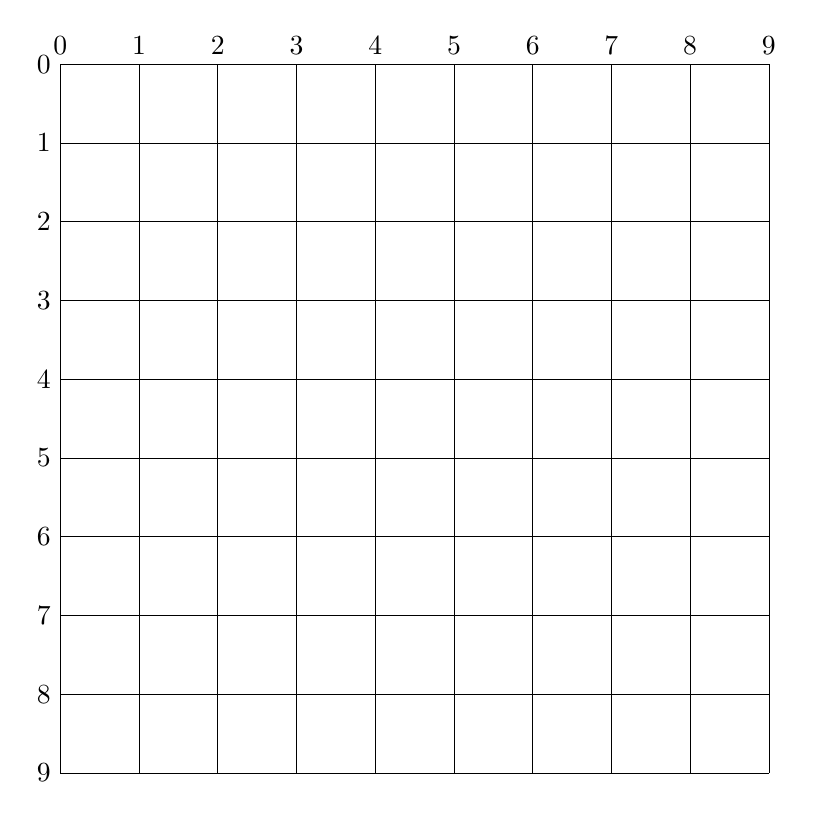
\begin{tikzpicture}
   \foreach \i in {0,...,9} {
      \draw [very thin,black] (\i,0) -- (\i,9)  node [above] at (\i,9) {$\i$};
    }
    \foreach \i in {0,...,9} {
       \draw [very thin,black] (0,\i) -- (9,\i) node [left] at (0,9-\i) {$\i$};
    }
\end{tikzpicture}

\end{document}
